\section{Diskussion}

\subsection{Teststrecke 1}

Durch die eingebauten Funktionen wurde ersichtlich, dass bei der Berechnung der Zeit bisher die Steigung als entscheidender Faktor nicht betrachtet wurde.
Auf der ersten Teststrecke muss das Löschfahrzeug insgesammt einen Höhenunterschied von ungefähr 70 Metern überwinden (Abb. \ref{profile}).
Über die hälfte der Distanz hat dabei eine Steigung von 1-3$\%$ und auf einem Viertel der Strecke sogar eine Steigung von 4-6$\%$ Ein Fahrzeug dieser Gewichtsklasse kann auf dieser Strecke folglich nicht die für den größten Teil dieses Anstiegs geltende Maximalgeschwindigkeit von 80 km/h erreichen.


\begin{figure}[h]
\centering
\begin{subfigure}{0.80\textwidth}
\centering
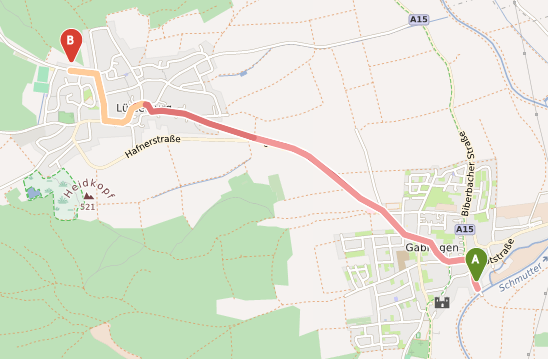
\includegraphics[width = \textwidth]{../media/Fahrt1_Steep.png} \\
\caption{Strecke 1 mit Steigung}
\label{fig:steig}
\end{subfigure}
\begin{subfigure}{0.18\textwidth}
\centering
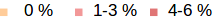
\includegraphics[width =0.60 \textwidth]{../media/legend2.png} \\
\caption{Legende}
\label{fig:legend2}
\end{subfigure}
\begin{subfigure}{ \textwidth}
\centering
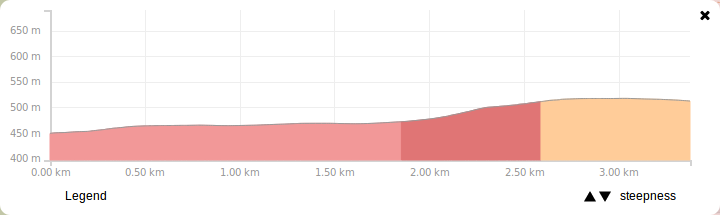
\includegraphics[width = \textwidth]{../media/Fahrt1_Profile.png} \\
\vspace{0.1cm}
\caption{Höhenprofil der ersten Strecke}
\label{profile}
\end{subfigure}
\caption{Steigung und Höhenprofil der ersten Teststrecke}
\label{steig}
\end{figure}

Darüber hinaus liegen auf der Strecke im inneren Lützelburgs ein paar langezogene aber dennoch scharfe Kurven (\ref{fig:turn}).
Auch hier kann das Löschfahrzeug nicht die gegebene Geschwindigkeit beibehalten und muss abbremsen.
Diese Kurven werden allerdings vom Emergency Profil nicht als Turn erkannt, da der Winkel zwischen den Segmenten zu groß ist.
Daher absolviert das Profil diesen Streckenabschnitt in geringerer Zeit als das echte Fahrzeug.

Weiterhin wurde bei allen drei Fahrten beobachtet, dass auf den Segmenten mit Maximalgeschwindigkeit (80 km/h) das Profil ebenfalls konstant ein paar Sekunden gegenüber der Testfahrt gutmachen kann.
Die Vermutung liegt nahe, dass das Löschfahrzeug die angegebene Maximalgeschwindigkeit nicht komplett erreichen kann.
Möglicherweise stimmt die Angabe sogar mit der Tachoanzeige überein aber die effektive Geschwindigkeit ist geringer.

Die Zeitdifferenzen aus Tabelle \ref{tab:all} zeigen: das Emergency-Profil fährt dem echten Fahrzeug mit der derzeitigen Gewichtung über die ganze Strecke hinweg davon.
Wenn die genannten Faktoren der Steigung, der nicht miteinberechneten schärferen Kurven und der Maximalgeschwindigkeit mit einbezogen werden, ist ein Ergebnis im 5 Minuten Bereich zu erwarten.


\subsection{Teststrecke 2}

Da die 2. Strecke nur in der Ebene verläuft sind keine Abweichungen durch die Steigung zu erwarten.
Die Differenzzeiten sind auch für alle fünf Wegpunkte ungefähr im +-10ß-Sekunden-Bereich.
Auffallend ist der Sprung vom 3. zum 4. Wegpunkt, bei welchem das Profil 14 Sekunden aufholt.
Nach einer genaueren Betrachtung dieses Segments stellte sich heraus, dass hier eine einspurige Unterführung durchfahren werden musste auf die eine durch die Topologie unübersichtliche Kurve folgt (Abb. \ref{fig:traintunnel}).
Vermutlich kam es daher auf der Fahrt zu Verzögerungen, was das Aufholen erklären könnte.

\begin{figure}[h]
\centering
\caption{Fahrt 2 -- Unterführung}
\label{fig:traintunnel}
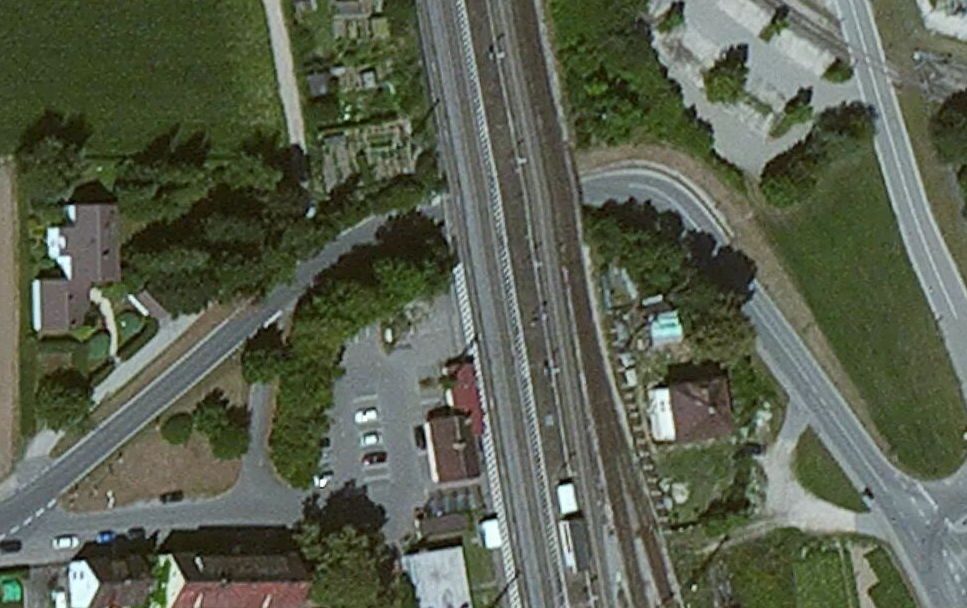
\includegraphics[width = 0.70 \textwidth]{../media/traintunnel.png} \\
\end{figure}


\subsection{Teststrecke 3}

Bei den Ergebnissen der 3. Strecke (Tab. \ref{tab:all}) ist das Profil bereits nach dem ersten Wegpunkt um mehr als 10 Sekunden zu langsam.
Bis zum Zwei-Minuten-Wegpunkt wird dieser Rückstand fast verdoppelt.
Nach genauerer Überprüfung der Durchschnittsgeschwindigkeiten stellte sich heraus, dass der Weg hier durch eine 30er-Zone führt.
Allerdings wird diese nicht mit den erwarteten 50 km/h sondern nur mit den durch den \texttt{maxspeed} Tag festgelegten 30 km/h durchfahren.
Offensichtlich ein Bug im Backend der noch behoben werden muss.

\begin{figure}[h]
\centering
\caption{Fahrt 3 -- Tempo-30-Zone}
\label{fig:temp30}
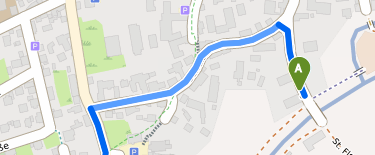
\includegraphics[width = 0.60 \textwidth]{../media/Fahrt3_temp30.png} \\
\end{figure}

Die anfängliche 30er-Zone ist fast 350m lang.
Diese Strecke kann in 25,2 Sekunden mit 50 km/h und in 42 Sekunden mit 30 km/h durchfahren werden.
Wird die Differenz von 16.8 Sekunden von den bisherigen Abweichungen für die 3. Fahrt abgezogen, werden die neuen Werte aus Tabelle \ref{tab:new3} erhalten.

\begin{table}[h]
\centering
\caption{Fahrt 3 -- neue Fahrzeit}
\label{tab:new3}
\begin{tabular}{|l|r|r|}
\hline
Wegpunkt & Sekunden & Abweichung \\ \hline 
1min & 70.8\footnote{Zum ersten Wegpunkt beträgt die Strecke nur 260m weshalb hier nur 12.6 Sekunden abgezogen werden} & -1.8  \\
2min & 139.4 & +2.6  \\
3min & 190 & -6.8  \\
4min & 255.2 & -1.6  \\
5min & 12.9 & -3.9  \\
\hline
\end{tabular}
\end{table}

Vor der 2 Minuten Marke beginnt eine Überlandstraße, die bis kurz vor Holzhausen (zwischen Marker 3 und 4) reicht.
Das sind 56$\%$ der Gesamtstrecke.
Wie bei der Diskussion der 1. Fahrt bereits erwähnt ist zu erwarten, dass die Maximalgeschwindigkeit von 80km/h ein bisschen zu hoch gegriffen ist, was den leichten Vorsprung zur 3-Minuten-Marke erklären könnte.

\begin{figure}[h]
\centering
\caption{Fahrt 3 -- Vergleich eines Turns}
\label{fig:turn}
\begin{subfigure}{0.49\textwidth}
\centering
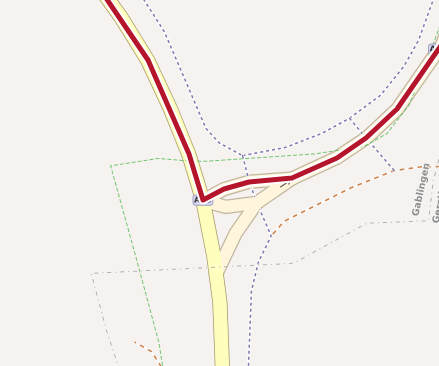
\includegraphics[width = 0.80\textwidth]{../media/Fahrt3_Turn.png} \\
\caption{Turn in den OSM Daten}
\label{fig:turnosm}
\end{subfigure}
\begin{subfigure}{0.49\textwidth}
\centering
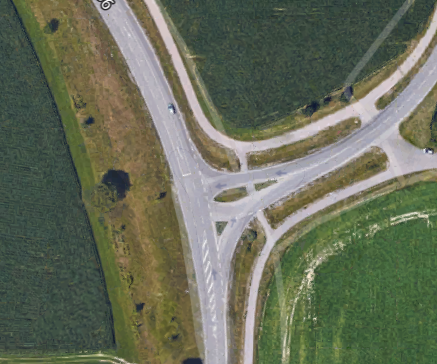
\includegraphics[width = 0.80\textwidth]{../media/Fahrt3_actualturn.png} \\
\caption{Turn in der Wirklichkeit}
\label{fig:turnworld}
\end{subfigure}
\end{figure}

Zwischen Punkt 3 und 4 fällt das Emergency Profil wieder um 5 Sekunden zurück.
Zwischen diesen Punkten befindet sich ein Turn, der deutlich schneller als andere Abbiegungen gefahren werden kann.
Abbildung \ref{fig:turn} zeigt einen Vergleich dieses Turns zwischen den OSM Daten(\ref{fig:turnosm}) und der eigentlichen Straße(\ref{fig:turnworld}).
Es ist zu erkennen, dass der Turn um einiges ''weicher'' ist als die Daten beschreiben.
Daher konnte das Löschfahrzeug gegenüber dem Profil Zeit gewinnen.

Schließlich zeigte auch diese Strecke nach einer Untersuchung des Höhenprofils einen Anstieg auf den letzten 150 Metern um 7-9$\%$(Abb. \ref{fig:profile2}) der noch nicht mit einberechnet wird und dem Emergency Profil wieder einen kleinen Vorsprung gibt.

\begin{figure}[h]
\centering
\caption{Fahrt 3 -- Höhenprofil}
\label{fig:profile2}
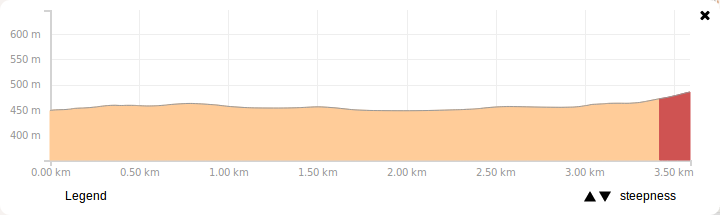
\includegraphics[width = 0.90 \textwidth]{../media/Fahrt3_Profile.png} \\
\end{figure}


\subsection{Benötigte Änderungen}

Wie durch die Vorliegende Analyse zu sehen ist, müssen noch einige Änderungen vollzogen werden, damit das Profil realistischere Ergebnisse zurückgibt.\par
\todo{liststyle}
Dass 30er Zonen noch nicht richtig erkannt werden muss repariert werden.
Für die Steigung muss auf jeden Fall noch eine Funktion implementiert werden, welche diese berücksichtigt.
Turns innerhalb von Routensegmenten, an Pillar Nodes, werden bisher nicht berücksichtigt.
Die Zeit für einen Turn sollte sowohl anhand des effektiven Winkels als auch anhand der Geschwindigkeiten des vorherigen und folgenden Wegsegmentes bestimmt werden.
Ansätze hierfür wurden bereits entwickelt(siehe Source Code) konnten aber noch nicht implementiert werden.
Für die Penalties sollte die Zeit, sofern vorhanden, aus der eigentlichen Beschleunigung und ansonsten möglicherweise aus dem Gewicht des Fahrzeugs berechnet werden.
Dadurch können einfacher spezifische Fahrzeugprofile erstellt und getestet werden.
Da das AccelerationWeighting sowohl für das Löschfahrzeug als auch für allgemeine Einsatzfahrzeuge benutzt wird, erhalten diese bisher die gleichen Penalties.
Das kann ebenfalls durch den zuletzt genannten Punkt behoben werden.
Weiterhin sollte für Einbahnstraßen die in Gegenrichtung durchfahren werden ein Penalty(ca. *0.9) gesetzt werden, da diese oft nicht mit der selben Geschwindigkeit durchfahren werden können wie in der eigentlichen Fahrtrichtung (auch wenn es erlaubt ist).
Das sollte ein Routing auf der Gegenfahrbahn wegen dem Gewinn von ein paar Sekunden verhindern.
Ebenfalls sollten dadurch eher vorhandene Parallelstraßen benutzt werden.